\documentclass[
	12pt,
	oneside,
	bibliography=totocnumbered]{scrartcl}


% For figures
\usepackage{graphicx}
\graphicspath{{./figures/}} % specify relative path with extra {}


% For references
\usepackage[
	backend=biber, % troubleshooting: http://tex.stackexchange.com/questions/154751/biblatex-with-biber-configuring-my-editor-to-avoid-undefined-citations
	style=numeric-comp]{biblatex}

\addbibresource{DFE_refs.bib}


% For hyperlinks in table of contents, and references
\usepackage{hyperref}
\hypersetup{
    colorlinks,
    citecolor=black,
    filecolor=black,
    linkcolor=black,
    urlcolor=black}


% General document info
\title{Terminating Information Search}
\author{Stefan Appelhoff}



%%%%%%%%%%%%%%%%%%%%%%%%%%%%%%%%%%%%%%%%%%%%%%%%%%%%%%%%%%%%%%


\begin{document}
\maketitle
\tableofcontents



\section{Introduction}

Selective Sampling

in that: Self-directed information search

best illustrated with an example ... laptop?

for the project described here, the aforementioned example will be transformed into an experimental paradigma that allows us to examine behavioral and neural aspects of choice in a controled manner.

Similar to the real life example, the experimental paradigms are characterized by:
- several options which can yield outcomes
- limited knowledge about the options and the frequencies of their associated outcomes
- opportunity to obtain information about the options via sampling
- the goal to maximize the positive outcomes obtained from the options

Through a structure of repeated sampling of the options and being provided with a feedback, the experimental paradigma describe sequential decision making problems.

In the trial to trial decisions participants make, the question of interest to this project lies in how participants set their stopping criteria. I.e., when do participants decide to terminate the information search in one option and switch to another option ... or stop sampling altogether. 

- See a concise formulation of the research questions in the *next section*.

- Afterwards, the details of the experimental paradigm will be outlined.

- Finally, the implementation of the experimental paradigm in terms of Matlab Code and Psychtoolbox will be described.





\section{Research Questions}
- How are sampling efforts sequentially allocated to the different options?

- How do we arrive at a decision to terminate the information search?

- What is the quantitative link between neural signals obtained by EEG with the behavioral data of participants performing the experimental paradigm. 






\section{The Experimental Paradigma}
In general, the experiment will be based on two different tasks that have been described in the literature previously. 

**name them**





\subsection{Bandit Paradigm}
for Hertwig (2009) also known as Partial-Feedback-Paradigm

\begin{figure}[h]
	\centering
	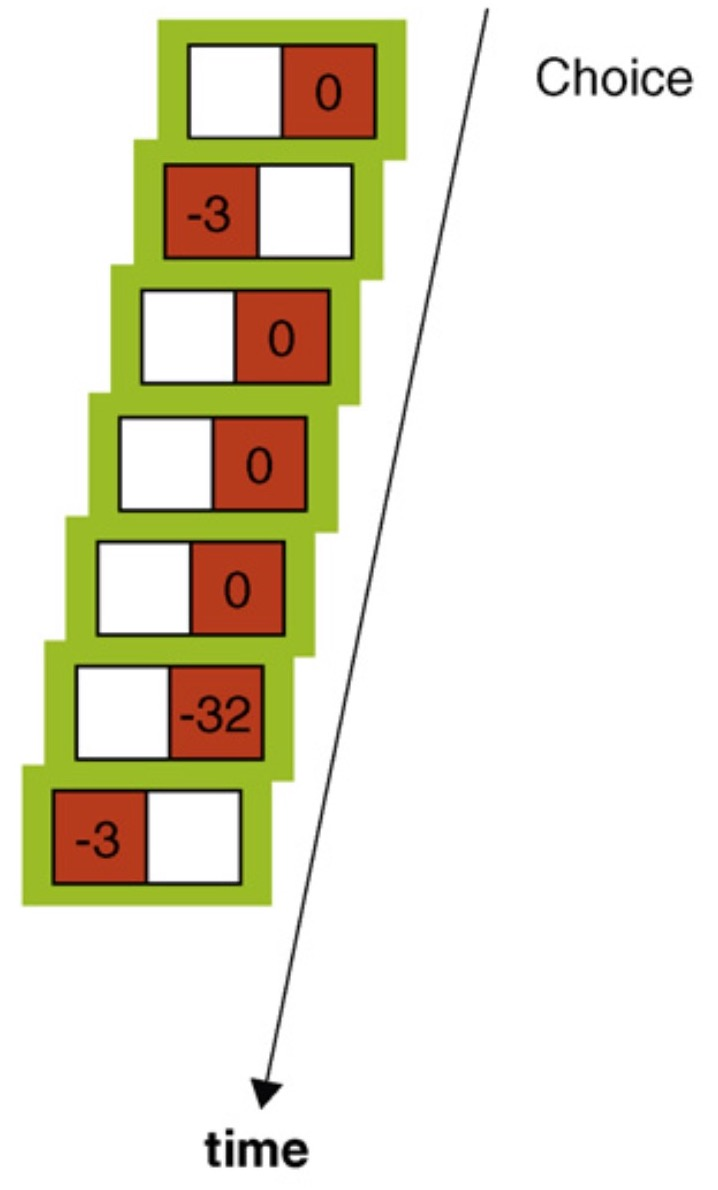
\includegraphics[scale=0.3]{pfp.jpg}
	\caption{Bandit Paradigm.}
	\label{fig:pfp}
\end{figure}

Figure \ref{fig:pfp} is adapted from XXX.




\subsection{Sampling Paradigm}
yep, pretty nice.


\begin{figure}[h]
	\centering
	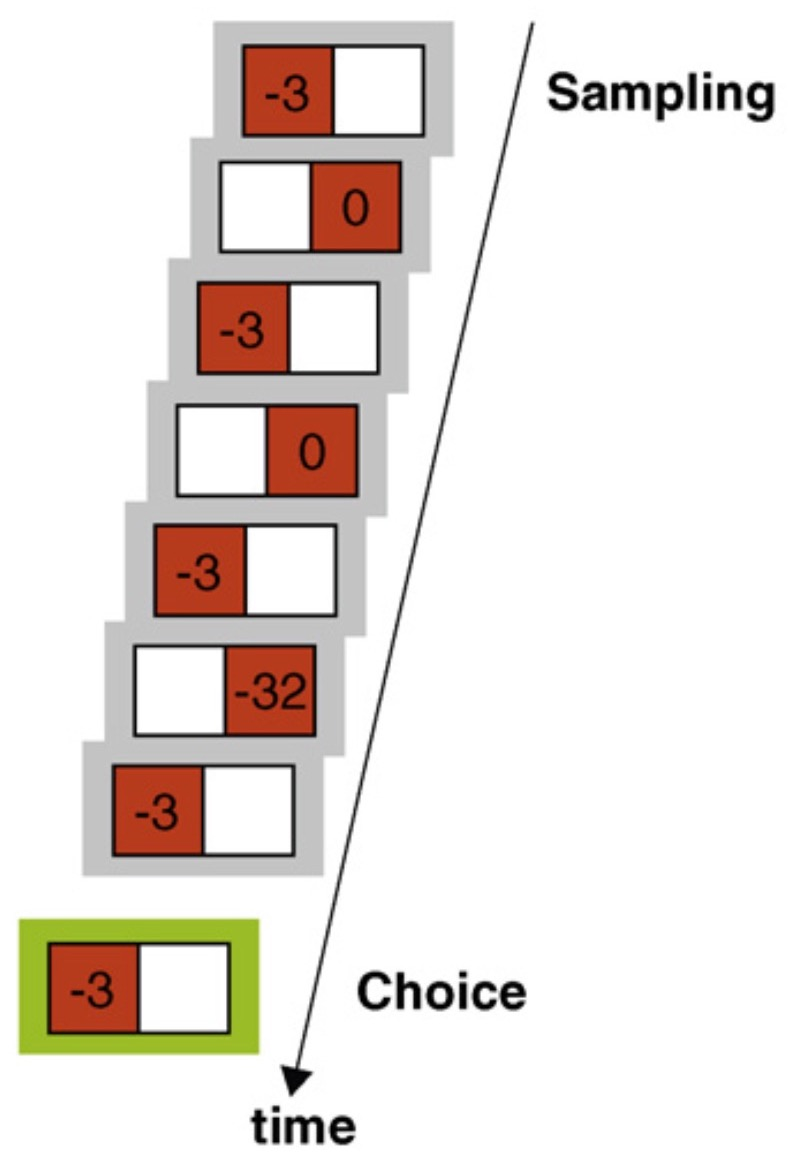
\includegraphics[scale=0.3]{sp.jpg}
	\caption{Sampling Paradigm.}
	\label{fig:sp}
\end{figure}

Figure \ref{fig:sp} is adapted from \cite{hertwig2009}.


\section{Computerized implementation of the Paradigma}
describe the computer code here


\printbibliography

\end{document}